% Figure 5: Predicted Throughput Comparison (GPU-only vs Hybrid)
% Standalone compilable: pdflatex fig5_throughput_bar.tex
\documentclass[border=5pt]{standalone}
\usepackage{tikz}
\usepackage{pgfplots}
\pgfplotsset{compat=1.18}

\begin{document}
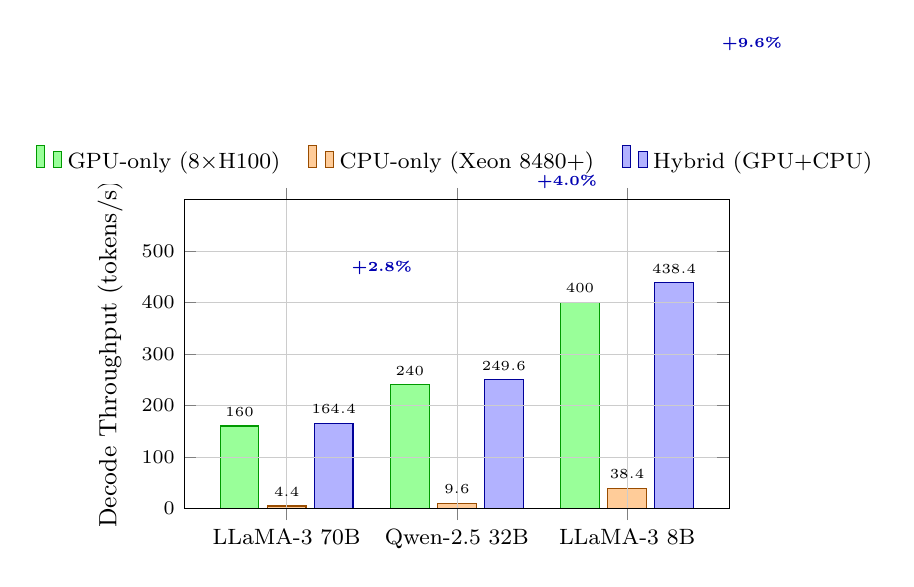
\begin{tikzpicture}
\begin{axis}[
    width=8.5cm,
    height=5.5cm,
    ybar=3pt,
    bar width=14pt,
    ylabel={Decode Throughput (tokens/s)},
    ylabel style={font=\small},
    xlabel style={font=\small},
    symbolic x coords={LLaMA-3 70B, Qwen-2.5 32B, LLaMA-3 8B},
    xtick=data,
    xticklabel style={font=\footnotesize, align=center},
    yticklabel style={font=\scriptsize},
    ymin=0, ymax=600,
    ytick={0, 100, 200, 300, 400, 500},
    legend style={
      at={(0.5,1.05)},
      anchor=south,
      legend columns=3,
      font=\footnotesize,
      draw=none,
      /tikz/every even column/.append style={column sep=8pt},
    },
    nodes near coords,
    every node near coord/.append style={font=\tiny, anchor=south},
    grid=major,
    grid style={line width=0.1pt, draw=gray!30},
    major grid style={line width=0.2pt, draw=gray!40},
    axis on top,
    enlarge x limits=0.3,
  ]

  % GPU-only throughput (mid-range estimates)
  \addplot[fill=green!40, draw=green!60!black] coordinates {
    (LLaMA-3 70B, 160)
    (Qwen-2.5 32B, 240)
    (LLaMA-3 8B, 400)
  };

  % CPU standalone throughput
  \addplot[fill=orange!40, draw=orange!60!black] coordinates {
    (LLaMA-3 70B, 4.4)
    (Qwen-2.5 32B, 9.6)
    (LLaMA-3 8B, 38.4)
  };

  % Hybrid throughput = GPU + CPU
  \addplot[fill=blue!30, draw=blue!60!black] coordinates {
    (LLaMA-3 70B, 164.4)
    (Qwen-2.5 32B, 249.6)
    (LLaMA-3 8B, 438.4)
  };

  \legend{GPU-only (8$\times$H100), CPU-only (Xeon 8480+), Hybrid (GPU+CPU)}

\end{axis}

% Gain annotations
\node[font=\tiny\bfseries, color=blue!70!black, anchor=west] at (2.0, 3.05) {+2.8\%};
\node[font=\tiny\bfseries, color=blue!70!black, anchor=west] at (4.35, 4.15) {+4.0\%};
\node[font=\tiny\bfseries, color=blue!70!black, anchor=west] at (6.7, 5.9) {+9.6\%};

\end{tikzpicture}
\end{document}
